\chapter{Introduzione}
La specifica della \textit{Prova Finale (Progetto di Reti Logiche)} 2021/2022 richiede di 
implementare un modulo Hardware descritto in VHDL che si interfacci con una
memoria con l'obiettivo di rappresentare un codificatore convoluzionale con tasso di trasmissione \( \frac{1}{2} \).
\section{Specifica del progetto}
Il modulo da implementare deve leggere la sequenza da codificare da una memoria, applicare la convoluzione parola per parola e 
successivamente salvare in memoria la sequenza codificata.
In particolare, dato un ordine, dovrà:
\begin{enumerate}
    \item Leggere la quantità di parole da codificare dalla memoria;
    \item Leggere la sequenza di parole da codificare una alla volta dalla memoria, ogni singola parola di memoria è un Byte;
    \item Trasformare la sequenza di Byte in un flusso di Bit (Serializzazione);
    \item Applicare al flusso di Bit il codice convoluzionale;
    \item Generare in uscita un flusso di Bit;
    \item Trasformare il flusso di Bit in Byte (Parallelizzazione);
    \item Salvare in memoria il risultato.
\end{enumerate}
Il tasso di trasmissione \( \frac{1}{2} \) indica che un Bit viene codificato con due Bit; infatti, il flusso 
in uscita è ottenuto come concatenamento alternato dei due Bit di uscita.

Il convolutore è una macchina sequenziale sincrona con un clock globale e un segnale di reset avente il diagramma 
degli stati come in \autoref{fig:Convolutore} e che ha nel suo 00 lo stato iniziale.
\begin{figure}
    \centering
    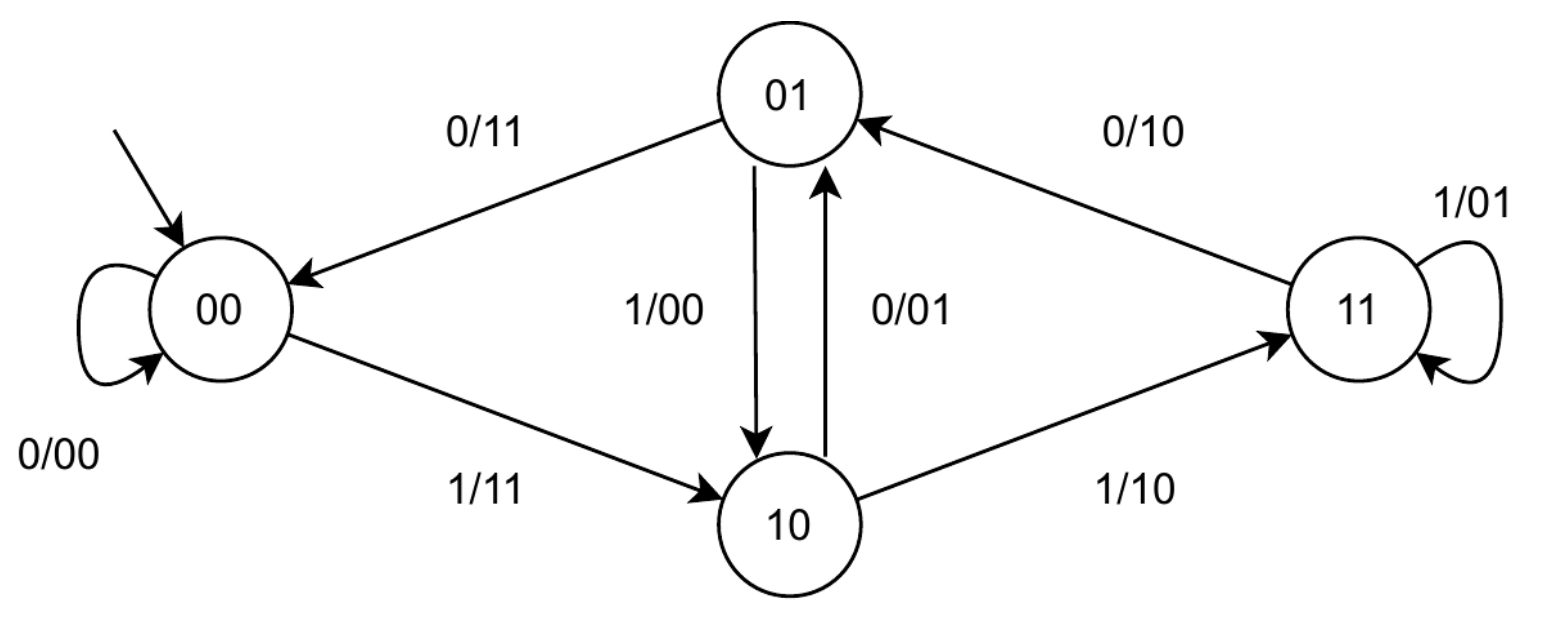
\includegraphics[width= 0.8\textwidth]{images/Capitolo1/conv.png} 
    \caption{Macchina a stati del codificatore convoluzionale} 
    \label{fig:Convolutore}
\end{figure}
\newpage
\section{Dati e dettagli}
\begin{itemize}
    \item Il modulo partirà nell'elaborazione quando un segnale \texttt{START} in ingresso verrà portato a 1.
    \item Il segnale di \texttt{START} rimarrà alto fino a che il segnale di \texttt{DONE} non verrà portato a 1.
    \item Al termine della computazione, il modulo da progettare deve portare a 1 il segnale \texttt{DONE} che notifica la fine dell’elaborazione e deve rimanere alto finché il segnale di \texttt{START} non è riportato a 0. 
    \item Un nuovo segnale \texttt{START} non può essere dato finché \texttt{DONE} non è stato riportato a 0. Se a questo punto viene rialzato il segnale di \texttt{START}, il modulo dovrà ripartire con la fase di codifica.
    \item Il modulo deve essere dunque progettato per poter codificare più flussi uno dopo l’altro. Ad ogni nuova elaborazione, il convolutore viene portato nel suo stato di iniziale 00.
    \item Il modulo deve essere progettato considerando che in una seconda elaborazione non dovrà attendere il \texttt{RESET} del modulo ma solo la terminazione dell'elaborazione.
\end{itemize}

\section{Struttura memoria}
La quantità di parole da codificare è memorizzata nell’indirizzo 0; il primo Byte (quindi la prima parola) della sequenza è memorizzato all’indirizzo 1. Le parole codificate in uscita devono essere memorizzate a partire dall’indirizzo 1000. La dimensione massima della sequenza di ingresso è 255 Byte.

\section{Interfaccia componente}
Il componente da descrivere ha un’interfaccia così definita:
\inputminted{vhdl}{listings/Capitolo1/componente.vhd}
In particolare:
\begin{itemize}
    \item \texttt{i\_clk} è il segnale di \texttt{CLOCK} in ingresso generato dal testbench;
    \item \texttt{i\_rst} è il segnale di \texttt{RESET} che inizializza la macchina pronta per ricevere il primo segnale di \texttt{START};
    \item \texttt{i\_start} è il segnale di \texttt{START} generato dal testbench;
    \item \texttt{i\_data} è il segnale che arriva dalla memoria in seguito ad una richiesta di lettura;
    \item \texttt{o\_address} è il segnale di uscita che manda l’indirizzo alla memoria;
    \item \texttt{o\_done} è il segnale di uscita che comunica la fine dell’elaborazione e il dato di uscita
    \item \texttt{o\_en} è il segnale di \texttt{ENABLE} da dover mandare alla memoria per poter comunicare
(sia in lettura che in scrittura);
    \item \texttt{o\_we} è il segnale di \texttt{WRITE ENABLE} da dover mandare alla memoria per poter scriverci. Per leggere da memoria esso deve essere 0;
    \item \texttt{o\_data} è il segnale di uscita dal componente verso la memoria.
scritto in memoria;
\end{itemize}